\documentclass[../header]{subfiles}

% \documentclass{standalone}
%
% \usepackage{tikz, ifthen}
% \usetikzlibrary{fit, matrix, positioning, shapes, decorations.pathreplacing,
%                 shapes.geometric, chains, arrows, calc }

% \newcommand{\mkContextPlane}[3][]{
%
% }

\begin{document}

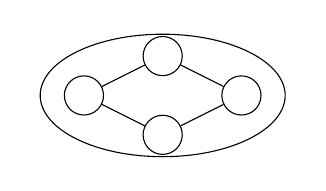
\begin{tikzpicture}[
  inf-piece/.style={draw, circle, inner sep=5pt}
  ]

\begin{scope}[yslant=-.5, xslant=1]%[yslant=-0.5, xslant=1]
  \node[inf-piece] (A) at (0,0) {};
  \node[inf-piece] (B) at (0,1) {};
  \node[inf-piece] (C) at (1,1) {};
  \node[inf-piece] (D) at (1,0) {};
  \draw[-] (A) -- (B) -- (C) -- (D) -- (A);
  \draw (.5,.5) ellipse (1.1);
  % \node[draw, ellipse, inner sep=0pt, fit=(A) (B) (C) (D)] {};
\end{scope}

\end{tikzpicture}

\end{document}
